\documentclass[final]{jpp}
\usepackage{graphicx}
%\usepackage[utf8]{inputenc}
\usepackage[T1]{fontenc}
\usepackage{amsmath}
\usepackage{bm}
\usepackage{natbib}
\usepackage{float}
\usepackage[colorlinks=true,
  linkcolor=black, citecolor=blue, urlcolor=blue]{hyperref}   % Modify colors of links
\usepackage[dvipsnames,svgnames,x11names,hyperref]{xcolor}  % Load colors for Tikz.
\usepackage[capitalize]{cleveref}
\input{mysty}

% Format citations
\crefformat{subsection}{\S#1}

\shorttitle{Non-Linear EPW}
\shortauthor{P. Cognet, B. J. Frei}

\title{Non-Linear Electron Plasma Waves in a Moment-Based Approach}

\author{P. Cognet \aff{1},B. J. Frei\aff{1}
  \corresp{\email{baptiste.frei@epfl.ch}}}

\affiliation{\aff{1} \'Ecole Polytechnique F\'ed\'erale de Lausanne (EPFL),
  Swiss Plasma Center,
CH-1015 Lausanne, Switzerland}

\begin{document}


\maketitle

\begin{abstract}
Abstract ...
\end{abstract}

\section{Introduction}

Electron Plasma waves occur when an electric field, in response to a small displacement of the electron density on the fixed ion background, pulls back the electron perturbation to its original position, yielding oscillations in the plasma density. The oscillations can interact with particle whose parallel velocity (parallel to the equilibrium magnetic field) is of the order of the phase velocity of the perturbation, yielding particle-wave interaction $\omega / k_\parallel \sim v_\parallel$. EPWs were predicted by the ground paper of \citet{Tonks1929} by deriving a dispersion relation. These types of waves are also known as "Langmuir" waves. From their dispersion relation, such waves propagate in a longitudinal direction with respect to the equilibrium magnetic field at a frequency just above the electron plasma frequency $\omega_{pe}^2 = 4 \pi n_{e0}e^2/m_e$. Moreover, \citet{Tonks1929} were also able to predict that these oscillations at lower frequencies are associated with what is known now as ion waves (or Ion accousitic waves) with a frequency such above the ion plasma frequency $\omega_{pi}^2 = 4 \pi n_{i0} e^2 / m_i$ (assuming an atomic number of $Z=1$). A theoretical work done by \citet{Landau1946} showed that the amplitude of EPWs decreases rapidly with its frequency $\omega$ using a Vlasov treatment of collisionless plasma. Instead of being dominated by energy transfer mechanism, the energy of the waves is scattered in velocity-space losing its spatial coherence. Moreover, EPWs are expected to exist for values of the wavenumber large that $1/\lambda_{De}$, i.e. $k \lambda_{De} < 1$. 

While EPW are electrostatic oscillations with a finite $k_\parallel$ have been extensively studied in the past and are a well-know plasma phenomena \citep{Tonks1929,Landau1946,ONeil1965,Jorge2019}, plasma oscillations perpendicular to a uniform externally imposed magnetic field in a warm plasma (i.e. with finite temperatire effects) is a much less studied subject. To this regard, we find that, in a fully ionized plasma, in which collisions are negligible, longitudinal electron oscillations propagating perpendicular to the equilibrium magnetic field exist, and gap in the allowed frequency spectrum at multiples of the electron gyrofrequency \citep{Bernstein1957}. This waves are the well-know Bernstein waves with $k_\parallel =0$ and $c^2 k^2/\omega^2 \ll 1$. The ion dynamics is included, coupling with the ion accoustic waves is expected. The subject of plasma oscillations in a magnetic field for which $k_\parallel =0$ is been the subject of \citep{Gross1950,Sen1952,Harris1959,Dory1965}. There, an $k\parallel =0$ unstable mode are reported in \citet{Dory1965} for finite $b = k_\perp v_\perp / \Omega_e$ values. In particular, broadening of the perpendicular equilibrium distribution function stabilizes the modes. This unstable modes can provides an efficient benchmark for kinetic Vlasov-Poisson continuum codes of magnetized plasmas \citep{Vogman2014}.


\section{Moment Hierarchy Equation}

We solve the drift-kinetic Boltzmann equation,

\begin{align} \label{eq:dFedt}
\pt \gyaver{\gyFe} + \dot \R\cdot \grad \gyaver{\gyFe} + \dot \vparallel \pvparallel \gyaver{\gyFe} =\gyaver{ C_{e}(\gyaver{\gyFe})},
\end{align}
\\
where $\dot \R = v_\parallel \b$, and $\dot \vparallel = e \grad_\parallel \phi/m_e$ using a Hermite decomposition for $\gyaver{\gyFe}$ for the parallel dynamics, i.e.

\begin{align}
\gyaver{\gyFe} = F_{eM} \sum_p N_e^p(\R,t) \frac{H_p(s_{\parallel e})}{\sqrt{2^p p!}},
\end{align}
\\
where the velocity variable is $s_{\parallel e} = \frac{v_\parallel-u_{\parallel e}(\R,t)}{v_{th \parallel e}(\R,t)}$ with $v_{th \parallel e}(\R,t) = \sqrt{2 T_{\parallel e}(\R,t)/m_e}$ and $u_{\parallel e}$ the drift velocity. The Maxwellian distribution is
\begin{equation}
F_{eM}(\vec{R},\vparallel,t)=N_e(\vec{R},t)\frac{1}{v_{th\parallel e}(\vec{R},t)\sqrt{\pi}}\exp\left[-\left(\frac{v_\parallel-u_{\parallel e}(\R,t)}{v_{th \parallel e}(\R,t)}\right)^2\right]    
\end{equation}{}
The Hermite polynomials $H_l$ are orthogonal over the interval $] -\infty, \infty[$ weighted by $e^{-x^2}$, such that

\begin{equation} \label{eq:Hermiteorthogonality}
    \int_{-\infty}^\infty d x H_l(x) H_{l'}(x) e^{-x^2} = 2^l l! \sqrt{\pi} \delta^l_{l'},
\end{equation}
\\
with $\delta_{l'}^l$ the Kronecker delta. From the previous relation, we derive that 

\begin{equation}
N_e N_e^p = 2 \pi \int d \mu d \vparallel \frac{B}{m_e} \gyaver{\gyFe} \frac{H_p(s_{\parallel e})}{\sqrt{2^p p!}}.
\end{equation}
\\
\Cref{eq:dFedt} is closed with the Poisson equation,

\begin{align}
\grad^2 \phi = 4 \pi e \left( N_{e} - \sum_iN_{i0}\right).
\end{align}


\section{Moment Hierarchy Equation Projection}

\begin{align}
2 \pi \int d \mu d \vparallel \frac{B}{m_e}\frac{H_l(s_{\parallel e})}{\sqrt{2^l l!}} \left[ \pt \gyaver{\gyFe} + v_\parallel \grad_\parallel \gyaver{\gyFe} + \frac{e}{m_e} \grad_\parallel \phi \pvparallel \gyaver{\gyFe} \right] =C_e^l,
\end{align}
\\
where $C_e^l = \int d \vi C_e H_l/(\sqrt{2^ll!})$. The intermediate results are 

\begin{align}
2 \pi &\int d \mu d \vparallel \frac{B}{m_e}\frac{H_l(s_{\parallel e})}{\sqrt{2^l l!}} \pt \gyaver{\gyFe}  \nonumber \\
=&\pt[\gyNe N_e^l]
+ \frac{\sqrt{2l}}{v_{th \parallel e}}  N_e N_e^{l-1} \frac{\partial u_{\parallel e}}{\partial t}
+ \frac{\partial (\ln T_{\parallel e})}{\partial t}  N_e \left[ \frac{l}{2}N_e^l+ \frac{\sqrt{l(l-1)}}{2}N_e^{l-2} \right],
\end{align}

\begin{align}
2 \pi &\int d \mu d \vparallel \frac{B}{m_e}\frac{H_l(s_{\parallel e})}{\sqrt{2^l l!}} v_\parallel \grad_\parallel \gyaver{\gyFe} \nonumber\\
 =&\frac{\partial}{\partial z}\left[  u_{\parallel e} N_e N_e^l + v_{th\parallel e} N_e\left(\sqrt{\frac{l+1}{2}} N_e^{l+1}+ \sqrt{\frac{l}{2}} N_e^{l-1}  \right) \right] \nonumber\\
&+ v_{th\parallel e} \frac{\partial (\ln T_{\parallel e})}{\partial z} N_e \left[  \frac{l}{2}\sqrt{\frac{l+1}{2}} N_e^{l+1}+\frac{l(2l-1)}{2\sqrt{2l}} N_e^{l-1} + \frac{\sqrt{l(l-1)(l-2)}}{2\sqrt{2}} N_e^{l-3}  \right] \nonumber\\
&+ u_{\parallel e} \frac{\partial (\ln T_{\parallel e})}{\partial z} N_e\left[ \frac{l}{2}N_e^l+ \frac{\sqrt{l(l-1)}}{2}N_e^{l-2} \right] \nonumber\\
&+ N_e\left( lN_e^l+ \sqrt{l(l-1)}N_e^{l-2}+ \frac{\sqrt{2l} u_{\parallel e}}{v_{th\parallel e}}N_e^{l-1}\right) \frac{\partial u_{\parallel e}}{\partial z},
\end{align}


\begin{align}
2 \pi &\int d \mu d \vparallel \frac{B}{m_e}\frac{H_l(s_{\parallel e})}{\sqrt{2^l l!}}  \frac{e}{m_e} \grad_\parallel \phi \pvparallel \gyaver{\gyFe} = - \frac{e}{m_e} \frac{\partial \phi}{\partial z} \frac{\sqrt{2l}}{v_{th\parallel e}} N_e N_e^{l-1},
\end{align} 

Giving the final result, in the order of $ \pt {N} $ followed by $\grad\cdot||\dot\R||$ then $ ||\dot v_\parallel||$ and two $\mathcal{F}$ terms,

\begin{align}
 &\pt[\gyNe N_e^l] \nonumber\\
 &+\frac{\partial}{\partial z}\left[ u_{\parallel e}N_eN_e^l +  v_{th\parallel e} N_e\left(\sqrt{\frac{l+1}{2}} N_e^{l+1}+ \sqrt{\frac{l}{2}} N_e^{l-1}  \right) \right] \nonumber\\
&- \frac{e}{m_e} \frac{\partial \phi}{\partial z} \frac{\sqrt{2l}}{v_{th\parallel e}} N_e N_e^{l-1}\nonumber\\
&+ \frac{\partial (\ln T_{\parallel e} )}{\partial t} N_e \left[ \frac{l}{2}N_e^l+ \frac{\sqrt{l(l-1)}}{2}  N_e^{l-2} \right] \nonumber\\
&+ v_{th\parallel e} \frac{\partial(\ln T_{\parallel e})}{\partial z}N_e \left[  \frac{l}{2}\sqrt{\frac{l+1}{2}} N_e^{l+1}+\frac{l(2l-1)}{2\sqrt{2l}} N_e^{l-1} + \frac{\sqrt{l(l-1)(l-2)}}{2\sqrt{2}} N_e^{l-3}  \right] \nonumber \\
&+ u_{\parallel e} \frac{\partial (\ln T_{\parallel e})}{\partial z} N_e\left[ \frac{l}{2}N_e^l+ \frac{\sqrt{l(l-1)}}{2}N_e^{l-2} \right] \nonumber\\
& + \frac{\sqrt{2l}}{v_{th \parallel e}}  N_e N_e^{l-1} \frac{\partial u_{\parallel e}}{\partial t} + N_e\left( lN_e^l +\sqrt{l(l-1)}N_e^{l-2}+  \frac{\sqrt{2l} u_{\parallel e}}{v_{th\parallel e}} N_e^{l-1} \right) \frac{\partial u_{\parallel e}}{\partial z} \nonumber\\
&= C_e^l 
\end{align}



\section{Normalization}
Normalized variables are used. The normalized density $ \hat{N}=\frac{N_e}{N_{e0}} $. The time $ \hat{t}=t \omega_{pe0} $ with $   \omega_{pe0}^2=\frac{4\pi N_{e0}e^2}{m_e} $. %meaning that $  \pt = \frac{1}{\omega_{pe}}\frac{\partial }{\partial t_{phys}} $.
The temperature $ \hat{T}=\frac{T_{\parallel e}}{T_{\parallel e0}} $. The position $ \hat{\R}=\frac{\R}{\lambda_{De0}} $ with $ \lambda_{De0}^2=\frac{T_{\parallel e0}}{4\pi N_{e0}e^2} $.
%Also $ \vec{x}=\vec{x}_{phys}/\lambda_{De} $, ($\lambda_{De}=4\pi N_e e^2/T_{e}$) so $ \frac{\partial}{\partial \vec{x}} = \lambda_{De} \frac{\partial}{\partial \vec{x}_{phys}} $ or $ \vec{x}=\vec{x}_{phys}/\rho_{Larmor,e} $, 
For the gyrocenter parallel fluid velocity use $ \hat{u}=\frac{u_{\parallel e}}{v_{th \parallel e}} $, noticing that the thermal velocity is $ v_{th \parallel e 0 }= \sqrt{\frac{2 T_{\parallel e0}}{m_e}} =  \lambda_{De0}\omega_{pe0}\sqrt{2 }$. %=\sqrt{\frac{T_{\parallel e0}}{4\pi N_{e0}e^2}\frac{4\pi N_{e0}e^2}{m_e}}=\sqrt{\frac{T_{\parallel e0}}{m_e}}= \frac{v_{th\parallel e0}}{\sqrt{2}} $, which is not consistent with used $ s_{\parallel e}=\frac{v_{\parallel e}}{v_{th\parallel e}} $. Note that $ v_{th\parallel e}=v_{th\parallel e0} \sqrt{\hat{T}_{\parallel e}} $.
The electric potential $ \hat{\phi}=\frac{e}{T_{\parallel e0}}\phi $. 


\begin{align}
 &\frac{\partial}{\partial \hat{t}}[\hat{N} N_e^l] \nonumber\\
 &+\sqrt{2} \frac{\partial}{\partial \hat{z}} \left( \hat{N} \hat{u}N_e^l\right) + \sqrt{l+1}  \frac{\partial}{\partial \hat{z}}  \left( \hat{N} \sqrt{\hat{T}}N_e^{l+1}\right)  + \sqrt{l}  \frac{\partial}{\partial \hat{z}}  \left( \hat{N} \sqrt{\hat{T}}N_e^{l-1}\right) 
 \nonumber\\
&-  \frac{\partial \hat{\phi}}{\partial \hat{z}} \sqrt{\frac{l}{ \hat{T}}} \hat{N} N_e^{l-1}\nonumber\\
&+ \frac{\partial  (\ln \hat{T} )}{\partial \hat{t}} \hat{N} \left[ \frac{l}{2}N_e^l+ \frac{\sqrt{l(l-1)}}{2}  N_e^{l-2} \right] \nonumber\\
&+ \sqrt{2\hat{T}}\frac{\partial (\ln \hat{T})}{\partial \hat{z}}\hat{N} \left(  \frac{l}{2}\sqrt{\frac{l+1}{2}} N_e^{l+1}+\frac{l(2l-1)}{2\sqrt{2l}} N_e^{l-1} + \frac{\sqrt{l(l-1)(l-2)}}{2\sqrt{2}} N_e^{l-3}  \right) \nonumber \\
&\;\;\;\;\;\;\;\;\;\;\;\;\;\;\;\;\;\;\;\;\;\;\;\;\;\;\; +  \sqrt{2}\frac{\partial (\ln \hat{T})}{\partial \hat{z}}\hat{N} \hat{u} \left(\frac{l}{2}N_e^l+  \frac{\sqrt{l(l-1)}}{2}N_e^{l-2} \right) \nonumber\\
& +  \sqrt{\frac{2l}{\hat{T}}} \hat{N}N_e^{l-1} \frac{\partial \hat{u}}{\partial \hat{t}}\nonumber\\
&+ \sqrt{2}\hat{N}\left( lN_e^l+ \sqrt{l(l-1)}N_e^{l-2} \right)\left(\frac{\partial \hat{u}}{\partial \hat{z}} \right) + 2  \hat{u} \sqrt{\frac{l}{\hat{T}}}  N_e^{l-1} \left(\frac{\partial \hat{u}}{\partial \hat{z}} \right) \nonumber\\
&= \frac{1}{\omega_{pe0}N_{e0}} C_e^l 
\end{align}

The only parameter left is $ \omega_{pe0}N_{e0} $. A more compact form is 
\begin{align}
\frac{\partial N_e^l}{\partial \hat{t}}= \mathcal{A}^l + \sum_p &\left[ \mathcal{B}_p^l \frac{\partial (\ln\hat{N})}{\partial \hat{t}} + \mathcal{C}_p^l  \frac{\partial (\ln\hat{N})}{\partial \hat{z}}+ \mathcal{D}_p^l \frac{\partial \hat\phi}{\partial \hat{z}}  + \mathcal{E}_p^l \frac{\partial (\ln \hat{T})}{\partial \hat{t}} + \mathcal{F}_p^l \frac{\partial (\ln\hat{T})}{\partial \hat{z}} \right. \nonumber\\
&\left. + \mathcal{G}_p^l \frac{\partial \hat{u}}{\partial \hat{t}} + \mathcal{H}_p^l  \frac{\partial \hat{u}}{\partial \hat{z}} \right]N_e^p +  \sum_p \mathcal{I}_p^l \frac{\partial N_e^p}{\partial\hat{z}}    \label{eq:time_evo_Nel}
\end{align}

\begin{align}
&\mathcal{A}^l=  \frac{C_e^l}{\omega_{pe0}N_{e0}\hat{N}}\\
&\mathcal{B}_p^l= -\delta_p^l\\
&\mathcal{C}_p^l=-\left(\sqrt{\hat{T}} \sqrt{l+1}\delta_p^{l+1}+ \sqrt{2}\hat{u} \delta_{p}^{l} +\sqrt{\hat{T}} \sqrt{l}\delta_p^{l-1} \right)\\
&\mathcal{D}_p^l=\sqrt{\frac{l}{\hat{T}}} \delta_p^{l-1} \\
&\mathcal{E}_p^l=- \frac{l}{2}\delta_p^l -\frac{\sqrt{l(l-1)}}{2}\delta_p^{l-2} \\
&\mathcal{F}_p^l=-\left[\sqrt{\hat{T}} \frac{(l+1)\sqrt{l+1}}{2} \delta_p^{l+1} + \frac{l}{\sqrt{2}} \delta_p^l  +\sqrt{\hat{T}}  l \sqrt{l}\delta_p^{l-1}\right. \nonumber\\
& \left.  \;\;\;\;\;\;\;\;\;\;\;\;\;\;\;\;\;\;+  \frac{\sqrt{l(l-1)}}{2}   \delta_p^{l-2}  + \sqrt{T} \frac{\sqrt{l(l-1)(l-2)}}{2} \delta_p^{l-3} \right] \\
&\mathcal{G}_p^l=- \sqrt{2l}\delta_p^{l-1} \nonumber\\
&\mathcal{H}_p^l=  - \sqrt{\hat{T}} \left( \sqrt{2}(l+1) \delta_p^l+ \hat{u}2\sqrt{\frac{l}{\hat{T}}}  \delta_p^{l-1} + \sqrt{2l(l-1)} \delta_p^{l-2} \right) \\
&\mathcal{I}_p^l=-\left(\sqrt{\hat{T}} \sqrt{l+1}\delta_p^{l+1}+\hat{u}\sqrt{2}\delta_p^l + \sqrt{\hat{T}} \sqrt{l}\delta_p^{l-1} \right)
%&\mathcal{B}_p^l= -\frac{\partial (\ln\hat{N})}{\partial \hat{t}}\delta_p^l -\frac{\partial (\ln \hat{N})}{\partial \hat{z}}\sqrt{\hat{T}}\left(\sqrt{l+1}\delta_p^{l+1}+ \hat{u}\sqrt{2} \delta_{p}^{l} +\sqrt{l}\delta_p^{l-1} \right) + \frac{\partial \hat{\phi}}{\partial\hat{z}}\sqrt{\frac{l}{\hat{T}}} \delta_p^{l-1} \nonumber\\
%&- \frac{\partial (\ln \hat{T})}{\partial \hat{t}}\left[ \frac{l}{2}\delta_p^l  + \hat{u}\sqrt{\frac{l}{2}} \delta_p^{l-1} +\frac{\sqrt{l(l-1)}}{2}\delta_p^{l-2} \right] - \frac{\partial (\ln\hat{T})}{\partial \hat{z}}\sqrt{\hat{T}}\left[ \frac{l\sqrt{l+1}}{2} \delta_p^{l+1} \right.\nonumber \\
%&+ \left. \hat{u}\sqrt{2}l \delta_p^l  +  \frac{\sqrt{l}(2l-1+2\hat{u}^2)}{2}\delta_p^{l-1} +  \sqrt{2l(l-1)}   \delta_p^{l-2} + \frac{\sqrt{l(l-1)(l-2)}}{2} \delta_p^{l-3} \right] \nonumber\\
%&- \frac{\partial \hat{u}}{\partial\hat{t}}\sqrt{2l}\delta_p^{l-1}
%- \frac{\partial \hat{u}}{\partial \hat{z}} \sqrt{\hat{T}} \left( \sqrt{2}l \delta_p^l+ \hat{u}2\sqrt{l}  \delta_p^{l-1} + \sqrt{2l(l-1)} \delta_p^{l-2} \right) \\
%\end{align}
%or 
%\begin{align}
%\mathcal{B}_p^l &=
%-\sqrt{\hat{T}(l+1)}\left( \frac{\partial (\ln \hat{N})}{\partial \hat{z}} + \frac{\partial (\ln\hat{T})}{\partial \hat{z}}\frac{l}{2} \right) \delta_p^{l+1}
%- \left( \frac{\partial(\ln\hat{T}_{\parallel e})}{\partial \hat{t}} \frac{l}{2} + \frac{\partial(\ln\hat{N}_{e})}{\partial \hat{t}}  \right) \delta_p^l \nonumber\\
%&+ \left[ -\sqrt{\hat{T}_{\parallel e}l} \left( \frac{\partial (\ln \hat{N}_e)}{\partial \hat{z}} + \frac{\partial (\ln \hat{T}_{\parallel e})}{\partial \hat{z}} \frac{2l-1}{2}  \right) + \frac{\partial\hat{\phi}}{\partial \hat{z}}\sqrt{\frac{l}{\hat{T}_{\parallel e}}} \right] \delta_p^{l-1} \nonumber \\
%&- \frac{\partial (\ln \hat{T}_{\parallel e})}{\partial \hat{t}} \frac{\sqrt{l(l-1)}}{2} \delta_p^{l-2} 
%- \frac{\partial (\ln\hat{T}_{\parallel e})}{\partial \hat{z}}\frac{\sqrt{\hat{T}_{\parallel e}l(l-1)(l-2)}}{2} \delta_p^{l-3} \\
%&\mathcal{C}_p^l=-\sqrt{\hat{T}}\left(\sqrt{l+1}\delta_p^{l+1}+     \hat{u}\sqrt{2}\delta_p^l   +\sqrt{l}\delta_p^{l-1}\right)
\end{align}

The Poisson equation becomes, using $ Z_{\rm eff}=\frac{\sum_i N_{i0}}{N_{e0}} $,
\begin{align}
    \label{eq:poisson}
    \frac{\partial^2\hat{\phi}}{\partial \hat{z}^2}=\hat{N}-Z_{\rm eff}.
\end{align}




\section{Time evolution of $\hat{N}$, $\hat{T}$ and $ \hat u $} \label{sec:timeEvol}

We compute the moments to get relation between the quantities.
\begin{align}
N_e N_e^0=2\pi \int d \mu d \vparallel \frac{B}{m_e}  \gyaver{\gyFe}\frac{1}{\sqrt{2^00!}} = N_e \;\Rightarrow \; N_e^0=1\\
N_eN_e^1=2\pi \int d \mu d \vparallel \frac{B}{m_e}  \gyaver{\gyFe}\frac{2 s_{\parallel e}}{\sqrt{2^11!}} %= N_e u_{\parallel e} \frac{1}{\lambda_{De0}\omega_{pe0}\sqrt{\hat{T}_{\parallel e}}}
\Rightarrow \; N_e^1=0\\%u_{\parallel e}=N_e^1\lambda_{De0}\omega_{pe0}\sqrt{\hat{T}_{\parallel e}} \\
N_eN_e^2=2\pi \int d \mu d \vparallel \frac{B}{m_e}  \gyaver{\gyFe}\frac{4 s_{\parallel e}^2-2}{\sqrt{2^22!}} \;\Rightarrow \; N_e^2=0  %\frac{(N_e^1)^2}{\sqrt{2}} \label{eq:link_N1_N2}
\end{align}

%$ N_e^3  $ linked to energy flux density?

Therefore $ N_e^0 $ is fixed, meaning that the time evolution equation (\ref{eq:time_evo_Nel}) for $ l=0 $ leads to an equation for the time evolution of $\hat{N}$ since there are no $\frac{\partial (\ln\hat{T})}{\partial \hat{t}}$ nor $\frac{\partial \hat{u}}{\partial \hat{t}}$ terms,
\begin{align}
    %\frac{\partial }{\partial \hat{t}}\hat{N}_e=\frac{C_e^0}{\omega_{pe0}N_{e0}}-\frac{\partial}{\partial \hat{z}}\left[\hat{N}_e \sqrt{\hat{T}_{\parallel e}}N_e^1\right].
    %\frac{\partial (\ln \hat{N})}{\partial \hat{t}}=\frac{C_e^0}{\omega_{pe0}N_{e0}\hat{N}}-\frac{\partial (\ln \hat{N})}{\partial \hat{z}} \sqrt{\hat{T}}N_e^1-\frac{\partial}{\partial \hat{z}}\left[\sqrt{\hat{T}}N_e^1\right].
    \frac{\partial (\ln \hat{N})}{\partial \hat{t}}=\frac{C_e^0}{\omega_{pe0}N_{e0}\hat{N}}-\frac{\partial (\ln \hat{N})}{\partial \hat{z}} \sqrt{2\hat{T}}\hat{u} -\frac{\partial (\ln \hat{T})}{\partial \hat{z}} \sqrt{\frac{\hat{T}}{2}}\hat{u} - \frac{\partial \hat{u}}{\partial \hat{z}}\sqrt{2\hat{T}} \label{eq:dlnNdt}.
\end{align}

Similarly equation (\ref{eq:time_evo_Nel}) for $l=2$ gives the time evolution for $\ln \hat T$ since there is no $\frac{\partial \hat{u}}{\partial \hat{t}}$ term,

\begin{align}
    \frac{\partial(\ln \hat T)}{\partial \hat t} =& 
    \frac{\sqrt{2}C_e^2}{\omega_{pe0}N_{e0}\hat{N}}
    -\sqrt{6\hat{T}}N_e^3 \frac{\partial(\ln\hat{N})}{\partial \hat{z}}
    -\sqrt{\hat{T}}\left(3\sqrt{\frac{3}{2}}N_e^3+2\sqrt{2}\hat{u}\right)\frac{\partial(\ln \hat{T})}{\partial \hat{z}} \nonumber\\
    &- 2\sqrt{2\hat{T}} \frac{\partial \hat{u}}{\partial \hat{z}} 
    - \sqrt{6\hat{T}} \frac{\partial N_e^3}{\partial\hat{z}} \label{eq:dlnTdt}.
\end{align}

Finally the time evolution for $\hat{u}$ is determined from equation (\ref{eq:time_evo_Nel}) with $l=1$. Note that the $\frac{\partial (\ln\hat{T})}{\partial \hat{t}}$ can be computed from equation (\ref{eq:dlnTdt}).

\begin{align}
    \frac{\partial \hat{u}}{\partial \hat t} =& 
    \frac{C_e^1}{\sqrt{2}\omega_{pe0}N_{e0}\hat{N}}
    -\sqrt{\frac{\hat{T}}{2}} \frac{\partial(\ln\hat{N})}{\partial \hat{z}}
    +\frac{1}{\sqrt{2\hat{T}}}\frac{\partial \hat{\phi}}{\partial \hat{z}}
    - \frac{\hat{u}}{2}  \frac{\partial (\ln\hat{T})}{\partial \hat{t}} \nonumber \\
    &-\frac{\sqrt{\hat{T}}(1+\hat{u}^2)}{\sqrt{2}} \frac{\partial(\ln \hat{T})}{\partial \hat{z}}
    - \sqrt{2\hat{T}} \hat{u} \frac{\partial \hat{u}}{\partial \hat{z}}
    \label{eq:dudt}.
\end{align}


%To get a time evolution equation for $\hat{T}$, we use the fact that $N_e^1$ and $N_e^2$ are linked by equation (\ref{eq:link_N1_N2}), meaning that equations (\ref{eq:time_evo_Nel}) for $l=1$ and $l=2$ are dependent.

%(For $l=1$ we have:)
%\begin{align}
    %&\hat{N}_e\frac{\partial }{\partial \hat{t}}N_e^1 +N_e^1
    %\left[\frac{C_e^0}{\omega_{pe0}N_{e0}}-\frac{\partial}{\partial \hat{z}}\left[\hat{N}_e \sqrt{\hat{T}_{\parallel e}}N_e^1\right]\right]
    %\frac{\partial }{\partial \hat{t}}\hat{N}_e
    %+ \frac{\partial}{\partial \hat{z}}\left[\sqrt{\hat{T}_{\parallel e}}\hat{N}_e\left((N_e^1)^2+1\right)\right] 
    %- \frac{\partial \hat{\phi}}{\partial \hat{z}} \frac{\hat{N}_e}{\sqrt{\hat{T}_{\parallel e}}} \nonumber\\
    %&+ \frac{\partial }{\partial \hat{t}}(\ln \hat{T}_{\parallel e})\frac{\hat{N}_e N_e^1}{2} 
    %+\frac{1}{2}\sqrt{\hat{T}_{\parallel e}} \frac{\partial}{\partial \hat{z}}(\ln \hat{T}_{\parallel e})\hat{N}_e \left((N_e^1)^2+1\right)= \frac{C_e^1}{\omega_{pe0}N_{e0}}
    
%    &\frac{\partial N_e^1}{\partial \hat{t}} =
%    - N_e^1 \frac{\partial(\ln \hat{N}_e) }{\partial \hat{t}}
%    - \frac{\partial}{\partial \hat{z}}\left[\sqrt{\hat{T}_{\parallel e}}\left(\sqrt{2}N_e^2+1\right)\right]
%    - \frac{\partial (\ln \hat{N}_e)}{\partial \hat{z}}\sqrt{\hat{T}_{\parallel e}}\left(\sqrt{2}N_e^2+1\right)
%    + \frac{\partial \hat{\phi}}{\partial \hat{z}} \frac{1}{\sqrt{\hat{T}_{\parallel e}}} \nonumber\\
%    &- \frac{\partial (\ln \hat{T}_{\parallel e})}{\partial \hat{t}}\frac{N_e^1}{2} 
%    -\frac{1}{2}\sqrt{\hat{T}_{\parallel e}} \frac{\partial (\ln \hat{T}_{\parallel e})}{\partial \hat{z}} \left(\sqrt{2}N_e^2+1\right)
%    +\frac{C_e^1}{\omega_{pe0}N_{e0}\hat{N}_e}
%\end{align}

%(For $l=2$ we have:)

%\begin{align}
%    &\frac{\partial N_e^2}{\partial \hat{t}} =
%    - N_e^2 \frac{\partial(\ln \hat{N}_e) }{\partial \hat{t}}
%    - \frac{\partial}{\partial \hat{z}}\left[\sqrt{\hat{T}_{\parallel e}}\left(\sqrt{3}N_e^3+\sqrt{2}N_e^1\right)\right]
%    - \frac{\partial (\ln \hat{N}_e)}{\partial \hat{z}}\sqrt{\hat{T}_{\parallel e}}\left(\sqrt{3}N_e^3+\sqrt{2}N_e^1\right) \nonumber\\
%    &+ \frac{\partial \hat{\phi}}{\partial \hat{z}} \sqrt{\frac{2}{\hat{T}_{\parallel e}}}N_e^1 
%    - \frac{\partial (\ln \hat{T}_{\parallel e})}{\partial \hat{t}}\left[ N_e^2 + \frac{1}{\sqrt{2}}  \right]
%    -\sqrt{\hat{T}_{\parallel e}} \frac{\partial (\ln \hat{T}_{\parallel e})}{\partial \hat{z}} \left(\sqrt{3}N_e^3+ \frac{3}{\sqrt{2}} N_e^1\right)
%    +\frac{C_e^2}{\omega_{pe0}N_{e0}\hat{N}_e}
%\end{align}

%Resulting in 
%\begin{align}
%    \frac{\partial (\ln \hat{T}_{\parallel e})}{\partial \hat{t}}&= \nonumber\\
%    \sqrt{2}&\left\{- N_e^2 \frac{\partial(\ln \hat{N}_e) }{\partial \hat{t}}
%    - \frac{\partial}{\partial \hat{z}}\left[\sqrt{\hat{T}_{\parallel e}}\left(\sqrt{3}N_e^3+\sqrt{2}N_e^1\right)\right]
%    - \frac{\partial (\ln \hat{N}_e)}{\partial \hat{z}}\sqrt{\hat{T}_{\parallel e}}\left(\sqrt{3}N_e^3+\sqrt{2}N_e^1\right) \right. \nonumber\\
%    &+ \frac{\partial \hat{\phi}}{\partial \hat{z}} \sqrt{\frac{2}{\hat{T}_{\parallel e}}}N_e^1 
%    -\sqrt{\hat{T}_{\parallel e}} \frac{\partial (\ln \hat{T}_{\parallel e})}{\partial \hat{z}} \left(\sqrt{3}N_e^3+ \frac{3}{\sqrt{2}} N_e^1\right)
%    \left. +\frac{C_e^2}{\omega_{pe0}N_{e0}\hat{N}_e} \right\} \nonumber\\
%    -2N_e^1& \left\{
%    - N_e^1 \frac{\partial(\ln \hat{N}_e) }{\partial \hat{t}}
%    - \frac{\partial}{\partial \hat{z}}\left[\sqrt{\hat{T}_{\parallel e}}\left(\sqrt{2}N_e^2+1\right)\right]
%    - \frac{\partial (\ln \hat{N}_e)}{\partial \hat{z}}\sqrt{\hat{T}_{\parallel e}}\left(\sqrt{2}N_e^2+1\right) \right. \nonumber\\ 
%    &\left.+ \frac{\partial \hat{\phi}}{\partial \hat{z}} \frac{1}{\sqrt{\hat{T}_{\parallel e}}} 
%    -\frac{1}{2}\sqrt{\hat{T}_{\parallel e}} \frac{\partial (\ln \hat{T}_{\parallel e})}{\partial \hat{z}} \left(\sqrt{2}N_e^2+1\right)
%    +\frac{C_e^1}{\omega_{pe0}N_{e0}\hat{N}_e} \right\}
%\end{align}

%It depends on the time derivative $\frac{\partial (\ln \hat{N}_e)}{\partial \hat{t}}$ which is known. Using both $\frac{\partial (\ln \hat{N}_e)}{\partial \hat{t}}$ and $\frac{\partial (\ln \hat{T}_{\parallel e})}{\partial \hat{t}}$ we can now compute the right hand side of equation (\ref{eq:time_evo_Nel}).
%NOT THIS
%\begin{align}
%    \frac{\partial }{\partial \hat{t}}(\ln \hat{T}_{\parallel e})\frac{\hat{N}_e}{\sqrt{2}} + \sqrt{2} N_e^1
%    \left\{
%    - \frac{\partial}{\partial \hat{z}}\left[\sqrt{\hat{T}_{\parallel  e}}\hat{N}_e\left((N_e^2)^2+1\right)\right] 
%    + \frac{\partial \hat{\phi}}{\partial \hat{z}} \frac{\hat{N}_e}{\sqrt{\hat{T}_{\parallel e}}} \right. \nonumber \\
%    \left. -\frac{1}{2}\sqrt{\hat{T}_{\parallel e}} \frac{\partial}{\partial \hat{z}}(\ln \hat{T}_{\parallel e})\hat{N}_e \left((N_e^1)^2+1\right) 
%    + \frac{C_e^1}{\omega_{pe0}N_{e0}} 
%    \right\}\nonumber \\
%    -\frac{(N_e^1)^2}{\sqrt{2}} \left[ \frac{C_e^0}{\omega_{pe0}N_{e0}}-
%    \frac{\partial}{\partial \hat{z}}\left[\hat{N}_e \sqrt{\hat{T}_{\parallel e}}N_e^1\right] \right] 
%    + \frac{\partial }{\partial \hat{z}}\left[ \sqrt{2\hat{T}_{\parallel e}} \hat{N}_e(\sqrt{\frac{3}{2}}N_e^3+N_e^1) \right] \nonumber\\
%    -\frac{\partial\hat{\phi}}{\partial\hat{z}}\sqrt{\frac{2}{T_{\parallel e}}}N_e^1 
%    +\sqrt{2\hat{T}_{\parallel e}} \frac{\partial}{\partial \hat{z}}\left(\ln \hat{T}_{\parallel e}\right) \hat{N}_e \left[ \sqrt{\frac{3}{2}}N_e^3+\frac{3}{2} N_e^1 \right]
%    = \frac{C_e^2}{\omega_{ep0}N_{e0}}
%\end{align}

%BUT THIS INSTEAD
%\begin{align}
%    \frac{\partial }{\partial \hat{t}}(\ln \hat{T}_{\parallel e})\frac{\hat{N}_e}{\sqrt{2}} \left( (N_e^1)^2+1 \right) + \sqrt{2}N_e^1 \hat{N}_e \frac{\partial N_e^1}{\partial \hat{t}} +\frac{1}{\sqrt{2}}(N_e^1)^2  \nonumber \\
%    -\frac{(N_e^1)^2}{\sqrt{2}} \left[ \frac{C_e^0}{\omega_{pe0}N_{e0}}-
%    \frac{\partial}{\partial \hat{z}}\left[\hat{N}_e \sqrt{\hat{T}_{\parallel e}}N_e^1\right] \right] 
%    + \frac{\partial }{\partial \hat{z}}\left[ \sqrt{2\hat{T}_{\parallel e}} \hat{N}_e(\sqrt{\frac{3}{2}}N_e^3+N_e^1) \right] \nonumber\\
%    -\frac{\partial\hat{\phi}}{\partial\hat{z}}\sqrt{\frac{2}{T_{\parallel e}}}N_e^1 
%    +\sqrt{2\hat{T}_{\parallel e}} \frac{\partial}{\partial \hat{z}}\left(\ln \hat{T}_{\parallel e}\right) \hat{N}_e \left[ \sqrt{\frac{3}{2}}N_e^3+\frac{3}{2} N_e^1 \right]
%    = \frac{C_e^2}{\omega_{ep0}N_{e0}}
%\end{align}


\section{Collisions}
The Lenard-Bernstein collision operator is 
\begin{equation}
    C_e = \nu \frac{\partial }{\partial v_\parallel}\left[v_\parallel \gyaver{\gyFe} + \frac{T_e}{m_e} \frac{\partial \gyaver{\gyFe}}{\partial v_\parallel} \right].
\end{equation}{}
It means that 
\begin{align}
    C_e^p &= 2 \pi \int d \mu d \vparallel \frac{B}{m_e} \frac{H_p(s_{\parallel e})}{\sqrt{2^p p!}}
           \nu \left[\gyaver{\gyFe} + \vparallel \frac{\partial \gyaver{\gyFe}}{\partial v_\parallel} + \frac{T_e}{m_e} \frac{\partial^2 \gyaver{\gyFe}}{\partial v_\parallel^2} \right] \nonumber \\
    &= \nu p N_e N_e^p - \nu \sqrt{2p} \frac{u_{\parallel e}}{v_{th \parallel e}} N_e N_e^{p-1}
\end{align}{}
After normalization
\begin{equation}
     \mathcal{A}^p = \frac{C_e^p}{\omega_{pe0}N_{e0}\hat{N}} = -\hat{\nu} p N_e^p - \hat{\nu} \sqrt{2p} \hat{u} N_e^{p-1},
\end{equation}{}
where $\hat{\nu} = \frac{\nu}{\omega_{pe0}}$ is a normalized collision frequency parameter provided by the user. Note that $\mathcal{A}^0=\mathcal{A}^2=0$ but $\mathcal{A}^1 = -\hat{\nu}\sqrt{2}\hat{u} $.

%$C_e^l\propto -l N_e^l$, meaning that  then $C_p^0=C_p^1=C_p^2=0$. For higher moments $l\geq3$, the formula used is
%\begin{align}
%\mathcal{A}^l=\frac{C_e^l}{\omega_{pe0}N_{e0}\hat{N}}= \frac{-\nu l N_e^l }{\hat{N}},
%\end{align}
%where parameter $\nu$ is a normalized collision frequency parameter provided by the user.



\section{Energies}
The potential field energy is (converting from SI units to Gaussian units)
\begin{align}
    E_{Pot} =& \frac{\epsilon_0}{2}\int_0^{z_{max}} E_{SI}^2(z)\; {\rm d}z \nonumber \\
    =& \frac{\epsilon_0}{2}\int_0^{z_{max}} \frac{1}{4\pi\epsilon_0} E^2(z)\; {\rm d}z \nonumber \\
    =& \frac{1}{8\pi}\int_0^{\hat{z}_{max}} \frac{1}{\lambda_{De0}^2} \left(\frac{\partial \phi(\hat{z})}{\partial \hat{z}} \right)^2 \; \lambda_{De0}{\rm d}\hat{z} \nonumber \\
    =& \frac{\lambda_{De0}}{8\pi}\int_0^{\hat{z}_{max}} \frac{T_{\parallel e0}^2}{\lambda_{De0}^2e^2} \left(\frac{\partial \hat{\phi}(\hat{z})}{\partial \hat{z}} \right)^2 \; {\rm d}\hat{z} \nonumber \\
    =& \frac{\lambda_{De0}}{8\pi}\int_0^{\hat{z}_{max}} \frac{4\pi N_{e0} e^2 T_{\parallel e0}^2}{T_{\parallel e0}e^2} \left(\frac{\partial \hat{\phi}(\hat{z})}{\partial \hat{z}} \right)^2 \; {\rm d}\hat{z} \nonumber \\
    =& \frac{\lambda_{De0}N_{e0}T_{\parallel e0}}{2}\int_0^{\hat{z}_{max}} \left(\frac{\partial \hat{\phi}(\hat{z})}{\partial \hat{z}} \right)^2 \; {\rm d}\hat{z}
\end{align}

The kinetic energy is
\begin{align}
    E_{kin} =& \frac{m_e}{2} \int_0^{z_{max}}{\rm d}z \int{\rm d}\vec{v} \; \vparallel^2  \gyaver{\gyFe} \nonumber \\
    =& \frac{m_e}{2} \int_0^{z_{max}}{\rm d}z \int{\rm d}\vec{v} \; (s_{\parallel e}v_{th \parallel e}+ u_{\parallel e})^2  \gyaver{\gyFe} \nonumber \\
    =& \frac{m_e}{2} \int_0^{z_{max}}{\rm d}z \int{\rm d}\vec{v} \; (s_{\parallel e}^2v_{th \parallel e}^2+ 2s_{\parallel e} v_{th \parallel e} u_{\parallel e}+ u_{\parallel e}^2)  \gyaver{\gyFe} \nonumber \\
    =& \frac{m_e}{2} \int_0^{z_{max}}{\rm d}z \int{\rm d}\vec{v} \; \left( \frac{v_{th \parallel e}^2}{4}\big(H_2(s_{\parallel e})+2\big)+ H_1(s_{\parallel e}) v_{th \parallel e} u_{\parallel e}+ u_{\parallel e}^2 \right)  \gyaver{\gyFe} \nonumber \\
    =& \frac{m_e}{2} \int_0^{z_{max}}{\rm d}z \; N_e\left( \frac{v_{th \parallel e}^2}{4}\big(2\sqrt{2}N_e^2 +2N_e^0\big)+  \sqrt{2}N_e^1 v_{th \parallel e} u_{\parallel e}+ N_e^0u_{\parallel e}^2 \right)  \nonumber \\
    =& \frac{m_e}{2} \int_0^{z_{max}}{\rm d}z \; N_e\left( \frac{v_{th \parallel e}^2}{2} + u_{\parallel e}^2 \right)  \nonumber \\
    =& \frac{m_e}{2} \int_0^{\hat{z}_{max}}{\rm d}\hat{z} \lambda_{De0} \; \hat{N}N_{e0} \frac{2\hat{T}T_{\parallel e 0}}{m_e} \left( \frac{1}{2} + \hat{u}^2 \right)  \nonumber \\
    =& \frac{\lambda_{De0} N_{e0} T_{\parallel e 0}}{2} \int_0^{\hat{z}_{max}}{\rm d}\hat{z}\; \hat{N} \hat{T} \left( 1 + 2\hat{u}^2 \right) \label{eq:Ekin}
\end{align}{}

The derivatives of the kinetic and potential energies are computed. If there are no collisions, the total energy is conserved as one expects.

For the kinetic energy, one can start use directly the drift-kinetic Boltzmann equation (\ref{eq:dFedt}), with no collisions ($C_e=0$) to get 

\begin{align}
    \pt E_{kin} =& \frac{m_e}{2} \int_0^{z_{max}}{\rm d}z \int{\rm d}\vec{v} \; \vparallel^2  \pt \gyaver{\gyFe} \nonumber \\
    =& \frac{m_e}{2} \int_0^{z_{max}}{\rm d}z \int{\rm d}\vec{v} \; \vparallel^2  \left( -v_\parallel \grad_\parallel \gyaver{\gyFe} - \frac{e}{m_e} \grad_\parallel \phi \pvparallel \gyaver{\gyFe} \right) \nonumber \\
    =&\dots  \nonumber \\
    =& \frac{\lambda_{De0} N_{e0} T_{\parallel e 0}\omega_{pe0}}{2} \int_0^{\hat{z}_{max}}{\rm d}\hat{z}  \left( 2\sqrt{2\hat{T}}\hat{N}\hat{u}  \frac{\partial \hat{\phi}}{\partial \hat{z} }  -  \frac{\partial}{\partial \hat{z}}[ \hat{T}^{3/2}\hat{N}(\sqrt{6}N_e^3+3\sqrt{2}\hat{u}+2\sqrt{2}\hat{u}^3) ]  \right)  \nonumber \\
    =& \frac{\lambda_{De0} N_{e0} T_{\parallel e 0}\omega_{pe0}}{2} \int_0^{\hat{z}_{max}}{\rm d}\hat{z} \; 2\sqrt{2\hat{T}}\hat{N}\hat{u}  \frac{\partial \hat{\phi}}{\partial \hat{z} } 
\end{align}{}

Another way to get to the same result is to start from equation (\ref{eq:Ekin}), then apply the derivatives of $ \hat T$, $ \hat N$ and $\hat u$ from section \ref{sec:timeEvol}, and setting the collisional terms to zero. This makes us more confident with the derivatives obtained in section \ref{sec:timeEvol}.

\begin{align}
    \pt E_{kin} =& \frac{\lambda_{De0} N_{e0} T_{\parallel e 0}\omega_{pe0}}{2} \int_0^{\hat{z}_{max}}{\rm d}\hat{z}\; \frac{\partial }{\partial \hat{t}} \left[ \hat{N} \hat{T} \left( 1 + 2\hat{u}^2 \right)\right] \nonumber \\
    =& \frac{\lambda_{De0} N_{e0} T_{\parallel e 0}\omega_{pe0}}{2} \int_0^{\hat{z}_{max}}{\rm d}\hat{z}\; \left[ \frac{\partial \hat{N}}{\partial \hat{t}} \hat{T} \left( 1 + 2\hat{u}^2 \right)  +  \hat{N} \frac{\partial \hat{T}}{\partial \hat{t}} \left( 1 + 2\hat{u}^2 \right) +\hat{N} \hat{T} 4 \frac{\partial \hat{u}}{\partial \hat{t}} \hat{u}  \right] \nonumber\\
    =& \;... \nonumber\\
    =& \frac{\lambda_{De0} N_{e0} T_{\parallel e 0}\omega_{pe0}}{2} \int_0^{\hat{z}_{max}}{\rm d}\hat{z}  \left( 2\sqrt{2\hat{T}}\hat{N}\hat{u}  \frac{\partial \hat{\phi}}{\partial \hat{z} }  -  \frac{\partial}{\partial \hat{z}}[ \hat{T}^{3/2}\hat{N}(\sqrt{6}N_e^3+3\sqrt{2}\hat{u}+2\sqrt{2}\hat{u}^3) ]  \right)  \nonumber \\
    =& \frac{\lambda_{De0} N_{e0} T_{\parallel e 0}\omega_{pe0}}{2} \int_0^{\hat{z}_{max}}{\rm d}\hat{z} \; 2\sqrt{2\hat{T}}\hat{N}\hat{u}  \frac{\partial \hat{\phi}}{\partial \hat{z} }    \label{eq:dEkin/dt}
\end{align}{}

To get the time derivative of the potential electromagnetic energy, Ampere's law is used, where the curl of the magnetic field is taken as zero.
\begin{align}
    \frac{\partial E_{Pot}}{\partial t} =& \frac{\epsilon_0}{2}\int_0^{z_{max}} {\rm d}z \;\frac{\partial}{\partial t}\big(E_{SI}^2\big) \nonumber \\
    =& \frac{\epsilon_0}{2}\int_0^{z_{max}} {\rm d}z \;2E_{SI}\frac{\partial E_{SI}}{\partial t} \nonumber \\
    =& \frac{\epsilon_0}{2}\int_0^{z_{max}} {\rm d}z \;2E_{SI}(-c^2\mu_0J_{SI}) \nonumber \\
    =& -\frac{1}{2}\int_0^{z_{max}} {\rm d}z \;2E_{SI}J_{SI} \nonumber \\
    =& -\frac{1}{2}\int_0^{z_{max}} {\rm d}z \;2\frac{E}{\sqrt{4\pi\epsilon_0}}J\sqrt{4\pi\epsilon_0} \nonumber \\
    =& -\frac{1}{2}\int_0^{\hat{z}_{max}} {\rm d}\hat{z}\lambda_{De0} \;2\left(\frac{\partial \hat{\phi}}{\partial \hat{z}} \frac{1}{\lambda_{De0}} \frac{T_{\parallel e0}}{e} \right) \left( e(\hat{N}N_{e0}) (v_{th\parallel e} \hat{u}) \right) \nonumber \\
    =& -\frac{1}{2}\int_0^{\hat{z}_{max}} {\rm d}\hat{z}\;     2\sqrt{2\hat{T}}\hat{N}\hat{u}  \frac{\partial \hat{\phi}}{\partial \hat{z} }   \label{eq:dEpot/dt}
\end{align}

So indeed without collisions the total energy is conserved 

\begin{align}
    \frac{\partial E}{\partial t} = \frac{\partial}{\partial t}(E_{Pot}+E_{Kin}) = 0
\end{align}

In our simulations, the potential energy is indeed following the expression on the right hand side of equation (\ref{eq:dEpot/dt}), but the kinetic energy doesn't follow the right hand side of equation (\ref{eq:dEkin/dt}), so the total energy is not conserved. \textbf{Further investigation is needed to find out why the kinetic energy doesn't behave correctly}.




%\section{Results TO BE UPDATED! MADE RUNNING OLD CODE}
%To check the validity the code, a simple run is performed to simulate the linear response in a fluid case. The temperature is set constant in space and frozen in time at $\forall \hat{z},\hat{t}$, $\hat{T}=1$. Similarly the moments are $\forall \hat{z},\hat{t}$, $N_e^0=1$ and $N_e^l=0$ for $l\geq1$. The periodic domain covered is $\hat{z}\in[0,z_{m}[$. Initially the perturbation is $\hat{N}=1+10^{-5}\cdot \sin(\frac{2\pi}{z_{m}} z)$, and $\hat{u}=0$. They then both evolves in time. Using these constraints, equations (\ref{eq:poisson}), (\ref{eq:dlnNdt}) and (\ref{eq:dudt}) can be linearized around the equilibrium values with periodic perturbations (eg $\hat{N}=1+e^{i(kz-\omega t)}\delta\hat{N}$) gives

%\begin{align}
%    &-k^2 \delta\hat{\phi}=\delta\hat{N}\\
%    & \omega\delta\hat{N}=\sqrt{2}k\delta\hat{u} \\
%    &\omega \delta\hat{u} = \frac{k}{\sqrt{2}}(\delta\hat{N}-\delta\hat{\phi})
%\end{align}
%This can be solve giving the dispersion relation
%\begin{align}
%    \omega = \sqrt{1+k^2} \;\;\Leftrightarrow\;\; \omega_{phys}=\omega_{pe0}\sqrt{1+(k_{phys}\lambda_{De0})^2} %T=\frac{2\pi}{\sqrt{1+\frac{4\pi^2}{z_m^2}}}
%\end{align}

%In our case the perturbation is $k=\frac{2\pi}{z_m}$. Figure \ref{fig:zm=1} shows that this oscillation frequency is indeed observed. 

%\begin{figure}
%    \centering
%    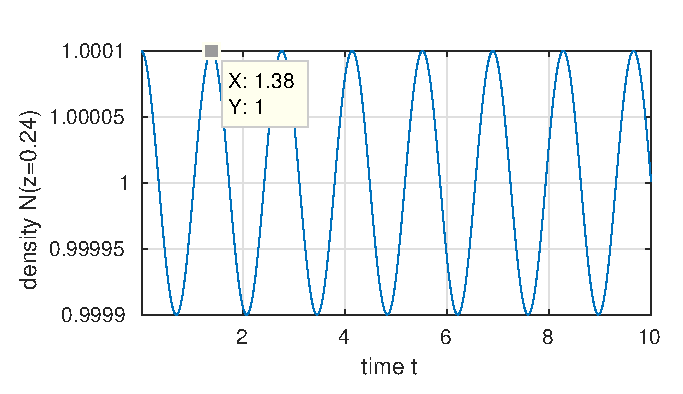
\includegraphics[width=0.5\textwidth]{zm1.eps}
%    \caption{Fluid approximation, undamped oscillation of density. Since $z_m=1$ the perturbation has $k=2\pi$ so the period $T= \frac{2\pi}{\sqrt{1+(2\pi)^2/2}} \approx1.3797$, as observed in the graph.}
%    \label{fig:zm=1}
%\end{figure}

%To further compare with the fluid model, a artificial damping term is added $-\nu \hat{u}$ to the right hand side of the equation (\ref{eq:dudt}), similarly to \cite{Banks2016} equation (39). This results indeed in a constant damped oscillations, again with frequency $\omega=\sqrt{1+k^2}$ and this time a damping rate of $\nu/2$ as shown in Figure \ref{fig:fluid_damping}. 

%\begin{figure}
%    \centering
%    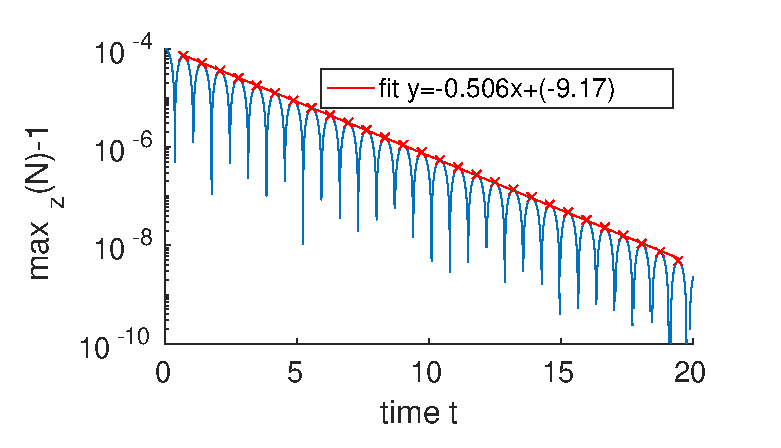
\includegraphics[width=0.5\textwidth]{fluid_damping.eps}
%    \caption{Fluid approximation, damped oscillation of density. Since $\nu=1$ the damping rate is $\nu/2$ as observed in graph.}
%    \label{fig:fluid_damping}
%\end{figure}
%Figures \ref{fig:moments} and \ref{fig:moments_2} show simulations with all fist 50 moments, and how a the perturbation is damped. In Figure \ref{fig:moments_2} we can see mutiple modes are present.
%\begin{figure}
%    \centering
%    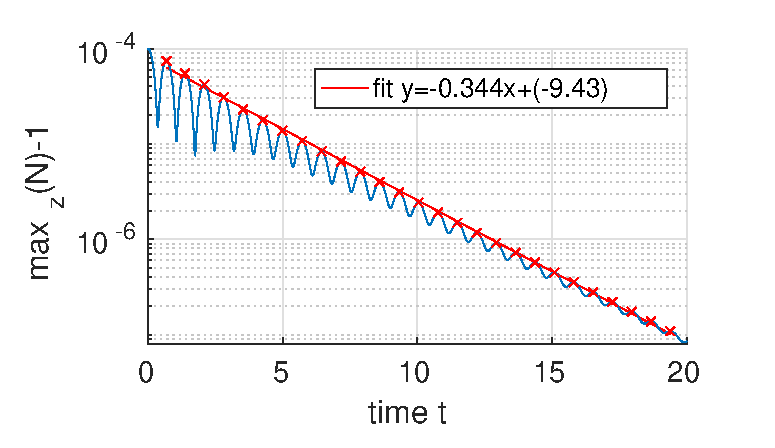
\includegraphics[width=0.5\textwidth]{moments.eps}
%    \caption{Full simulation with 50 moments, $\nu=0.1$ and $k=\frac{2\pi}{1}$.}
%    \label{fig:moments}
%\end{figure}

%\begin{figure}
%    \centering
%    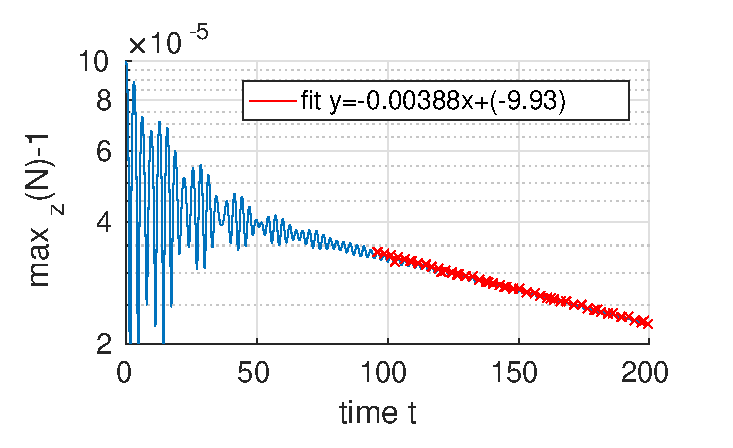
\includegraphics[width=0.5\textwidth]{moments_2.eps}
%    \caption{Full simulation with 50 moments, $\nu=0.01$ and $k=\frac{2\pi}{20}$.}
%    \label{fig:moments_2}
%\end{figure}

%%\begin{figure}
%%\centering
%%\includegraphics[width=0.1\linewidth]{zm=1.eps}
%%\caption{Period $T= %%\frac{2\pi}{\sqrt{1+(2\pi)^2/2}} \approx1.3797$}
%%\label{fig:zm=1}
%%\end{figure}


\bibliographystyle{jpp}
\bibliography{references}
\end{document}
 